\begin{frame}{Дисковая подсистема}

	\begin{block}{Блочное устройство}
		Вид файла устройств в UNIX/Linux-системах,  обеспечивающий интерфейс к устройству,
		реальному или виртуальному, в виде файла в файловой системе.
	\end{block}

	\begin{block}{Файловая система}
		Файловая система определяет формат содержимого и способ физического хранения информации,  
		которую принято группировать в виде файлов. 
		Конкретная файловая система определяет размер имени файла (директории),  
		максимальный возможный размер файла и раздела,  набор атрибутов файла.

		Распространенные для ОС Linux: ext2, ext4, xfs, reiserfs, vfat.
	\end{block}
\end{frame}

\begin{frame}{Примеры блочных устройств}

	\begin{itemize}
		\item {\tt /dev/{\bf s}d*}
		\item {\tt /dev/{\bf h}d*}
		\item {\tt /dev/ram*}
		\item {\tt /dev/loop*}
	\end{itemize}

	\begin{block}{Практическое задание:}
		\begin{enumerate}
			\item Посмотреть список вышеперечисленных устройств
			\item Посмотреть информацию об устройствах {\tt loop0, ram, sda}\\
				Hint: {\tt fdisk -l <device>}
		\end{enumerate}
	\end{block}
\end{frame}

\begin{frame}{Структура диска}
	\begin{columns}
		\column{0.6\textwidth}
		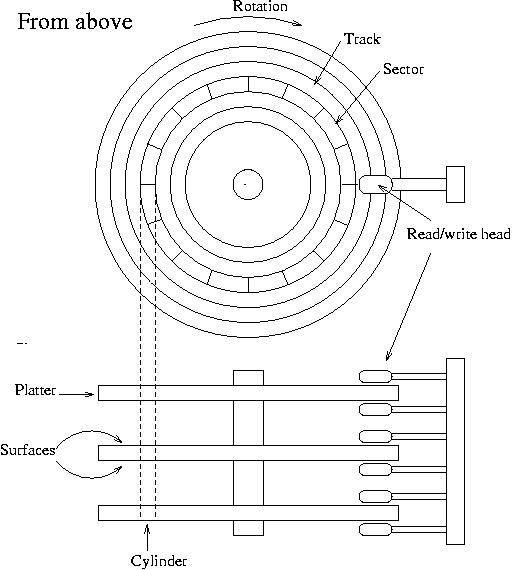
\includegraphics[height=0.8\textheight]{../../slides/disk/04-hd-schematic.png}
		\column{0.4\textwidth}
		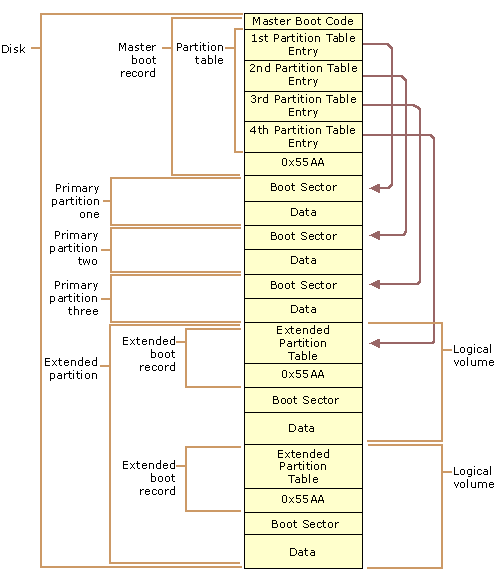
\includegraphics[height=0.8\textheight]{../../slides/disk/04-disk-structure.png}
	\end{columns}
\end{frame}

\begin{frame}{Отображение блочных устройств}


	\begin{block}{Device Mapper}
			{\tt /dev/mapper/*}\\
			device-mapper -- служит общим фреймворком для отображения одного блочного устройства на другое.

			Примеры: RAID, LVM, шифрованные диски и т.д.
	\end{block}

\end{frame}



